\documentclass[journal]{IEEEtran}

\usepackage[pdftex]{graphicx}
\usepackage{amsmath}
\usepackage{algorithmic}
\usepackage{cleveref}
\usepackage{url}

\begin{document}

\title{In-situ visualization of natural hazards with TACC Galaxy and Material Point Method}
\author{Greg Abram, %~\IEEEmembership{Fellow,~OSA,}
        Andrew Solis,
        and~Krishna Kumar% <-this % stops a space
\thanks{Department of Civil, Architectural and Environmental Engineering, University of Texas at Austin, TX, 78712 USA e-mail: (krishnak@utexas.edu).}% <-this % stops a space
\thanks{Texas Advanced Computing Center, University of Texas at Austin, TX,.}% <-this % stops a space
\thanks{Manuscript received September 3rd, 2021.}}

% The paper headers
\markboth{IEEE Computing in Science and Engineering (CiSE), Special Issue 2021}%
{}

%\IEEEpubid{0000--0000/00\$00.00~\copyright~2015 IEEE}
% use for special paper notices
%\IEEEspecialpapernotice{(Invited Paper)}

% make the title area
\maketitle

% As a general rule, do not put math, special symbols or citations
% in the abstract or keywords.
\begin{abstract}
The abstract goes here.
\end{abstract}

% Note that keywords are not normally used for peerreview papers.
\begin{IEEEkeywords}
In-situ viz, MPM, TACC-Galaxy.
\end{IEEEkeywords}

\IEEEpeerreviewmaketitle

\section{Overview and motivation}
% - why simulating earthquakes is important
% - why such sim is hard
% - brief description of MPM and benefits, cite to marker paper
% - why in situ vis is needed / benefits
% - Galaxy + MPM = awesomeness
\IEEEPARstart{L}{andslide} runouts are regional-scale events that can bury whole towns (e.g., 2018 Southern California mudflows that followed a series of wildfires~\cite{lukashov2019post}, 2014 Oso landslide caused 43 fatalities in the US) or devastate entire regions (e.g., 2016 Kaikoura, New Zealand earthquake recorded 100,000 landslides within a 12,000 sq. km area~\cite{dellow2017landslides}). The frequency of these regional-scale landslides is increasing with devastating earthquakes, extreme precipitation, and wildfires caused by climate change. Even in these risk-prone communities, where the residents are aware of the threat posed by the landslides, the residents repeatedly show indifference to these threats and consequently fail to act. The human capacity to deny danger endangers lives and property~\cite{kim2020public}. In 2020, twenty-two extreme events cost the United States \$95 billion in damages. The underlying problem is the uncertainty of the actual event and a lack of understanding of its potential impacts. How to communicate the reality of potential risk to a diverse group of individuals, who must understand and support a complex set of actions that reduce the risk for the whole community?
  
Visualization is the key to communicating scientific results effectively to engineering decision-makers and the public~\cite{mayer2005cognitive}. Given the limited cognitive capacity in humans, visualizing the complex threats as images enhances the brain's capacity to perceive opportunities and make decisions. Visual representation of complex information reduces the cognitive load on human information processing and increases human ``absorptive capacity" for problem-solving~\cite{kahneman2012human}. However, these visualizations must be physically sound to be perceived as realistic and accepted as valid.

Despite the landslide risks, most regional-scale landslide hazard analyses do not consider downstream impacts and the aerial extent of debris-flow runouts~\cite{USGS2017debris}. Traditional numerical methods such as the Finite Element Method (FEM) primarily focuses on the onset of failure but provides limited information on the post-failure runout mechanisms due to mesh distortions at large  deformations~\cite{soga2016trends}. Modeling the impacts of the potential runout of large landslides is possible with new tools such as Material Point Method (MPM)~\cite{Bardenhagen2000,Bardenhagen2004,Sulsky1994,Sulsky1995}. MPM is a mesh-free method that discretizes the domain as a collection of \textit{material points} moving on a background grid, and Newton's laws of motion determine their deformations. In this study, we employ the CB-Geo MPM code (\url{https://github.com/cb-geo/mpm}), and a typical MPM computation cycle is shown in~\cref{fig:mpm}. For more information on MPM and the code implementation, refer to~\cite{kumar2019scalable}. MPM results of the landslide runout can be translated into compelling visualizations to inform decision-makers of potential hazards. 

\begin{figure}[!htbp]
    \centering
    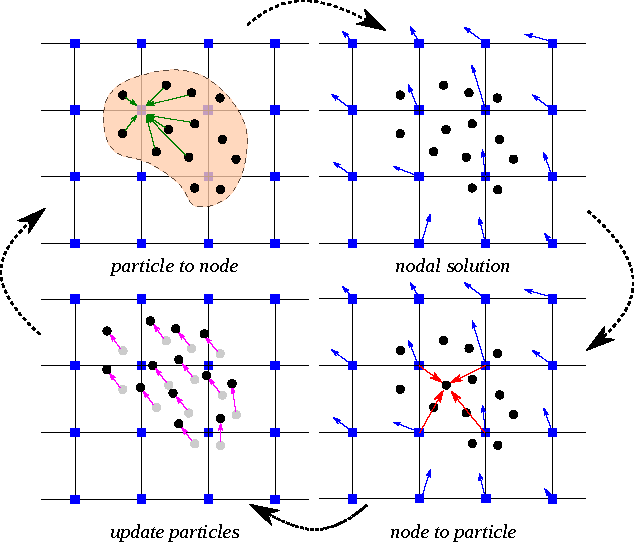
\includegraphics[width=\linewidth]{figs/mpm.pdf}
    \caption{Illustration of the MPM algorithm (1) A representation of material points overlaid on a computational grid. Arrows represent material point state vectors (e.g., mass, volume, and velocity) is projected to the nodes of the computational grid. (2) The equations of motion are solved onto the nodes, resulting in updated nodal velocities and positions. (3) The updated nodal kinematics is interpolated back to the material points. (4) The state of the material points is updated, and the computational grid is reset.}
    \label{fig:mpm}
\end{figure}

A regional-scale landslide simulation of a kilometer-scale runout with MPM requires billions of material points and millions of cells in the background grid. Scaling applications to simulate a billion particles require exascale high-performance computing (HPC) architectures with efficient Message-Passing Interface (MPI). This study uses the CB-Geo MPM code, which exploits a hybrid MPI+X approach to achieve regional-scale simulation of landslides. In addition, as the landslide runout progresses, the workload distributed across the compute nodes becomes imbalanced. We adopt a distributed graph-partitioning technique to load balance both the background mesh and particle distribution dynamically.

Visualization is also context and user-specific, i.e., different users may be interested in different aspects of the experimental or simulation data sets. Hence, the same data set may be represented in several forms – perhaps at varying levels of detail, emphasizing or deemphasizing different regions and features, and employing different visualization techniques to best present the information. Data retrieval and visualization in High-Performance Computing applications have long been a bottleneck. Current techniques for visualizing exascale simulations involve writing a temporal slice of a subset of the data to disk, often at a much coarser resolution than the original data, which leads to a significant portion of information being disregarded and potentially lost, followed by post-processing. In practice, this usually means that the data are stored only at specific time steps. An exascale simulation would output terabytes of data, resulting in a significant portion of the compute time spent on I/O~\cite{byna2020exahdf5}. Nevertheless, the scale of such discrete geometry visualization will push commercial rendering engines like Mantra and Arnold to the limit. The amount of data would be several orders of magnitude higher at exascale levels, making the simulation spend most of the compute time in I/O.

In-situ visualization is a rendering technique for visualizing the simulation data in real-time without requiring additional storage resources~\cite{abram2018galaxy,atzori2021situ,kress2019comparing}. Running the visualization and simulation in tandem avoids data transfer bottleneck, enabling scientists to monitor and modify simulation parameters in real-time. In-situ visualization libraries such as ParaView Catalyst and SENSEI offer the ability to couple existing data models (such as VTK) to query regions of interest and to render simulations. However, scaling rendering engines to exascale simulations remains a challenge requiring billions of lightpaths to be rendered. Most rendering engines only sample a limited number of random light paths can be at each step. Thus, the visual quality of rendered images suffers from estimator variance, which appears as visually distracting noise~\cite{yang2021foveated}. Ray tracing engines such as TACC Galaxy~\cite{abram2018galaxy} offer distributed asynchronous in-situ visualization capabilities for exascale simulations. In this study, we couple the CB-Geo MPM code with distributed asynchronous ray tracing engine TACC Galaxy to realize the 2014 Oso landslide in the US with 50 million material points.
  
\section{Related work}
  - brief summary other in situ, cite Hank term paper, maybe others

\section{Methodology}
\begin{itemize}
  \item tie into existing VTK-write path
  \item Galaxy expand to handle unstructured mesh
  \item tracking particles across domain boundaries
\end{itemize}
  
\section{Results}
  - show some pretty pictures
  - provide some runtime stats

\section{Conclusion}
- Future work

\appendices

% use section* for acknowledgment
\section*{Acknowledgment}
The authors would like to thank...


% Can use something like this to put references on a page
% by themselves when using endfloat and the captionsoff option.
\ifCLASSOPTIONcaptionsoff
  \newpage
\fi

% trigger a \newpage just before the given reference
% number - used to balance the columns on the last page
% adjust value as needed - may need to be readjusted if
% the document is modified later
%\IEEEtriggeratref{8}
% The "triggered" command can be changed if desired:
%\IEEEtriggercmd{\enlargethispage{-5in}}

% references section

% can use a bibliography generated by BibTeX as a .bbl file
% BibTeX documentation can be easily obtained at:
% http://mirror.ctan.org/biblio/bibtex/contrib/doc/
% The IEEEtran BibTeX style support page is at:
% http://www.michaelshell.org/tex/ieeetran/bibtex/
\bibliographystyle{IEEEtran}
% argument is your BibTeX string definitions and bibliography database(s)
\bibliography{IEEEabrv,references.bib}
%
% <OR> manually copy in the resultant .bbl file
% set second argument of \begin to the number of references
% (used to reserve space for the reference number labels box)
%\bibliography{references.bib}

% biography section
% 
% If you have an EPS/PDF photo (graphicx package needed) extra braces are
% needed around the contents of the optional argument to biography to prevent
% the LaTeX parser from getting confused when it sees the complicated
% \includegraphics command within an optional argument. (You could create
% your own custom macro containing the \includegraphics command to make things
% simpler here.)
%\begin{IEEEbiography}[{\includegraphics[width=1in,height=1.25in,clip,keepaspectratio]{mshell}}]{Michael Shell}
% or if you just want to reserve a space for a photo:

% \begin{IEEEbiography}{Michael Shell}
% Biography text here.
% \end{IEEEbiography}

% if you will not have a photo at all:
% \begin{IEEEbiographynophoto}{John Doe}
% Biography text here.
% \end{IEEEbiographynophoto}

%\vfill

% Can be used to pull up biographies so that the bottom of the last one
% is flush with the other column.
%\enlargethispage{-5in}
\end{document}


